\en

This chapter presents an overview of fundamental topics needed to understand 
the research, such as the Linux Kernel, refactoring, types of code duplication, 
code duplication detection methods presented in the literature and ways to 
evaluate these methods. This foundation will make it easier to grasp the 
concepts discussed in the research.

\section{The Linux Kernel}

The Linux kernel, a Unix-like operating system kernel, was published by Linus
Torvalds in 1992 as free software. It began gaining popularity in the late
1990s \citep{linuxbook}. Contrary to popular belief, Linux itself is not a
complete operating system, as it lacks components like filesystem utilities and
windowing systems. The so-called ``Linux distributions'' that are commonly
recognized by the public are actually GNU/Linux operating systems, which
include various essential applications alongside the Linux kernel,
such as system
\citep{gnuref}. Examples of Linux distributions are Ubuntu \citep{ubuntu} 
and Arch Linux \citep{archlinux}.

The Linux kernel is monolithic and organized into subsystems, such as
the process scheduler, memory management, device driver infrastructure,
networking, and filesystems \citep{melissa}. Each subsystem typically has a
dedicated maintainer or a team of maintainers responsible for overseeing its
development and managing contributions \citep{melissa}.

Development contributions to the Linux kernel are coordinated using the Git
version control system. These contributions are formatted as patches—text
documents that outline the differences between two source code versions.
These patches are then submitted and reviewed via the Linux mailing lists
\citep{melissa}.

Mailing lists are the primary means of communication within the Linux
community. Members of the community use them to submit and review patches,
discuss Linux-related topics, and debate potential new features. Given the
kernel's extensive modularity, each subsystem has its mailing list, allowing
discussions to be organized around specific areas of development
\citep{melissa}. All interactions on these mailing lists are documented and
archived in the Linux Kernel Lore \citep{linuxlore}, which serves as a
repository for kernel discussions and can be accessed by anyone interested.

One of the subsystems within the Linux kernel is the AMD Display driver, which
is responsible for implementing the drivers needed for AMD GPUs to function
correctly in a Linux environment. The maintainers of this subsystem have
reported a practical issue: a significant amount of duplicated code, which
complicates the maintenance of this subsystem. This problem serves as the
starting point for our research, with the AMD Display driver as our primary
object of study as we aim to understand and mitigate code duplication in the
Linux kernel. The AMD Display driver subsystem contains more then 391000 lines 
of code and more then 1089 code files
\footnote{ 
Data extracted directly from the Linux repository with the help of the cloc tool.
\citep{cloc}
}, 
making it a considerable component within the Linux kernel. Like other 
subsystems, discussions about the AMD Display driver are conducted on its 
designated mailing list, which can be accessed here: 
\url{https://lists.freedesktop.org/mailman/listinfo/amd-gfx}.

Another subsystem within the Linux kernel explored in this work is the
Industrial I/O subsystem (IIO). According to the Linux kernel documentation, 
''The main purpose of the Industrial I/O subsystem (IIO) is to provide support 
for devices that in some sense perform either analog-to-digital conversion (ADC) 
or digital-to-analog conversion (DAC) or both''\citep{iiodoc}. The IIO subsystem 
contains more than X lines of code and more than Y code files
\footnote{
Data extracted directly from the Linux repository with the help of the clol tool. \citep{cloc}
}.
We opted to include the IIO subsystem in our experiments to ensure our findings 
are not limited to one subsystem. Additionally, we have an established point of
contact within the IIO subsystem to facilitate this work.
Like other subsystems, discussions about the IIO subsytem are conducted on its 
designated mailing list, which can be found here: 
\url{https://subspace.kernel.org/vger.kernel.org.html}.


\subsection{Diff command}

The \textit{diff} command is a command line in Linux that allows the user to compare 
two files line by line \citep{diffcommand}. There are multiple forms in which the command 
results can be shown to the user, and Figure \ref{fig:diff} shows one of them. 
With the command results, it is easy to visualize and extract the number of lines that 
are equal and different between the two compared files.

\begin{figure}
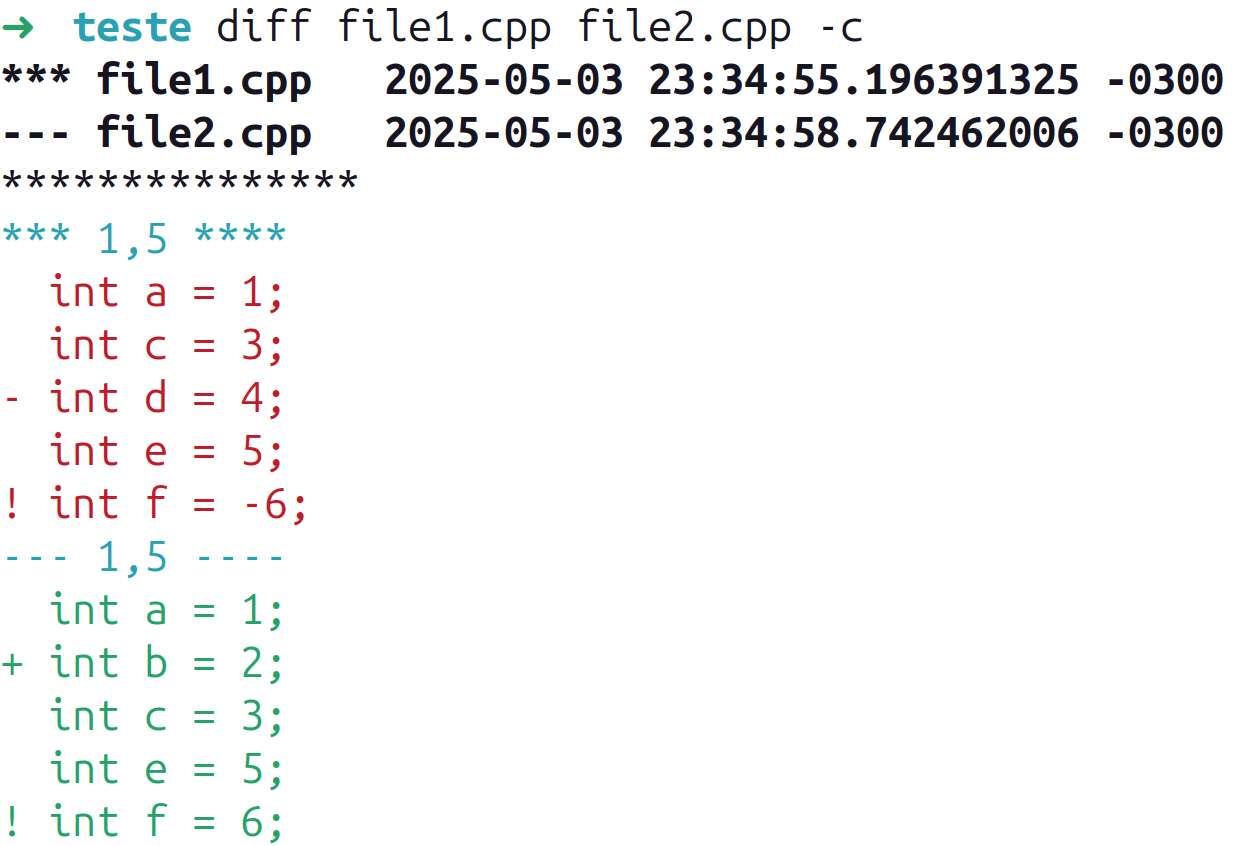
\includegraphics[scale=0.25]{diff_command}
\caption[Example of \textit{diff} command executed]{
Example of \textit{diff} command executed
\footnote{
File 1's content is shown in red, and file 2's content is shown in green. \textit{-} 
represents a line that only exists in file 1, \textit{+} represents a line that only 
exists in file 2,\textit{!} represents a line that exists in both files but has modifications 
between them, and empty at the start of a line represents that the line exists in 
both files without any modifications.
}
}
\label{fig:diff}
\end{figure}

We use the \textit{diff} command as the base of one of the code duplication detection 
methods on the tool proposed in this work, although it is not explored as the text 
similarity method for code duplication detection.
